% =====================================================================
% Semana 3 · S3.2 — Polarización por divisor de base
% Fundamentos de Sistemas Electrónicos Analógicos (Ingeniería Aeroespacial)
% Compilar: pdflatex semana_3_s32_divisor_base.tex  (2 pasadas)
% =====================================================================
\documentclass[aspectratio=169]{beamer}

\usepackage[utf8]{inputenc}
\usepackage[T1]{fontenc}
\usepackage{lmodern}
\usepackage[spanish,es-tabla]{babel}
\usepackage{amsmath,amssymb}
\usepackage{siunitx}
\usepackage{booktabs}
\usepackage{microtype}
\usepackage{circuitikz}

\definecolor{navy}{RGB}{23,54,93}
\definecolor{navysoft}{RGB}{72,101,140}
\definecolor{gold}{RGB}{179,142,62}
\definecolor{ink}{RGB}{44,51,58}
\definecolor{soft}{RGB}{244,241,234}

\usetheme{default}
\setbeamertemplate{navigation symbols}{}
\setbeamertemplate{footline}[frame number]
\setbeamercolor{structure}{fg=navy}
\setbeamercolor{frametitle}{fg=white,bg=navy}
\setbeamercolor{title}{fg=navy}
\setbeamercolor{subtitle}{fg=navysoft}
\setbeamercolor{itemize item}{fg=gold}
\setbeamercolor{itemize subitem}{fg=gold}
\setbeamercolor{block title}{fg=white,bg=navy}
\setbeamercolor{block body}{bg=soft}
\setbeamercolor{example text}{fg=navy}
\setbeamertemplate{itemize item}{\scriptsize\raise1.25pt\hbox{\donotcoloroutermaths$\bullet$}}
\setbeamertemplate{itemize subitem}{\scriptsize\raise1.25pt\hbox{\donotcoloroutermaths$\circ$}}
\setbeamerfont{frametitle}{size=\large,series=\bfseries}

\title[S3.2 · Divisor de base]{Polarización por divisor de base}
\subtitle{S3.2 — Simulaciones y laboratorio de la Semana 3}
\institute{Licenciatura en Ingeniería Aeroespacial\\ UNAM · ENES Unidad Juriquilla}
\author{M. en C. José de Jesús Santana Ramírez}
\date{Semestre 2027-1}

\begin{document}

% ---------------------------------------------------------------------
\begin{frame}[plain]
  \titlepage
\end{frame}

% ---------------------------------------------------------------------
\begin{frame}{Objetivos de la sesión}
  \begin{itemize}
    \item Aplicar el \textbf{equivalente de Thévenin} del divisor de base (conecta con S2.4).
    \item Calcular el punto Q con el divisor R1–R2 y el emisor $R_E$.
    \item Comprobar que esta topología \textbf{casi no depende de $\beta$} ni de la temperatura.
    \item Comparar con la polarización fija (S3.1).
  \end{itemize}
  \pause
  \begin{block}{Conexión con la Semana 2}
    El divisor de base se "ve" desde la base como una fuente de Thévenin: $V_{th}$ y $R_{th}$.
  \end{block}
\end{frame}

% ---------------------------------------------------------------------
\begin{frame}{Teoría 1 · El divisor de base con emisor}
  \begin{center}
    \resizebox{0.72\linewidth}{!}{%
    \begin{circuitikz}[american voltages, scale=1.0]
      \node[npn] (Q) at (4.4,1.6) {$Q$};
      \draw (0,0) to[V, l={$V_{CC}=12\,\mathrm{V}$}, i=$I$] (0,3.2);
      \draw (0,3.2) -- (7,3.2);
      \draw (0,0) -- (7,0);
      \node[ground] at (7,0) {};
      \draw (Q.C) to[R, l={$R_C=4.7\,\mathrm{k}$}] (7,3.2);
      \draw (Q.E) to[R, l={$R_E=1\,\mathrm{k}$}] (4.4,0);
      \draw (Q.B) -- (3.4,1.6);
      \draw (3.4,3.2) to[R, l={$R_1=47\,\mathrm{k}$}] (3.4,1.6);
      \draw (3.4,1.6) to[R, l={$R_2=10\,\mathrm{k}$}] (3.4,0);
    \end{circuitikz}}
  \end{center}
  \[
    V_{th} = V_{CC}\cdot\frac{R_2}{R_1+R_2}
    \qquad
    R_{th} = R_1\parallel R_2
  \]
\end{frame}

% ---------------------------------------------------------------------
\begin{frame}{Teoría 2 · Punto Q estable}
  Aplicando Thévenin en la base y $I_C \approx I_E$:
  \[
    I_E = \frac{V_{th}-V_{BE}}{R_E + R_{th}/\beta}
  \]
  \pause
  \begin{itemize}
    \item Si $R_E \gg R_{th}/\beta$ (o $\beta$ alto), entonces $I_E \approx \dfrac{V_{th}-V_{BE}}{R_E}$:
      \textbf{casi independiente de $\beta$}.
    \item La realimentación de $R_E$ compensa la variación de $V_{BE}$ y de $\beta$ (estabilidad térmica).
    \item $V_{CE} = V_{CC} - I_C(R_C + R_E)$.
  \end{itemize}
\end{frame}

% ---------------------------------------------------------------------
\begin{frame}{Ejercicio · Cálculo del punto Q}
  \begin{block}{Datos}
    \centering
    $V_{CC} = \SI{12}{\volt}$, $R_1 = 47\,\text{k}$, $R_2 = 10\,\text{k}$, $R_C = 4.7\,\text{k}$, $R_E = 1\,\text{k}$, $V_{BE} = \SI{0.7}{\volt}$, $\beta = 100$.
  \end{block}
  \[
    V_{th} = 12\cdot\frac{10}{57} = \SI{2.105}{\volt}
    \qquad
    R_{th} = 47\,\text{k}\parallel 10\,\text{k} = \SI{8.246}{\kilo\ohm}
  \]
  \[
    I_E = \frac{2.105 - 0.7}{1000 + 8246/100} = \frac{1.405}{1082.5} = \SI{1.298}{\milli\ampere}
  \]
  \[
    I_C \approx \SI{1.30}{\milli\ampere}
    \qquad
    V_{CE} = 12 - 1.30\,\text{mA}(4.7\,\text{k}+1\,\text{k}) = \SI{4.59}{\volt}
  \]
\end{frame}

% ---------------------------------------------------------------------
\begin{frame}{Resultado de la simulación · Estabilidad}
  \begin{center}
    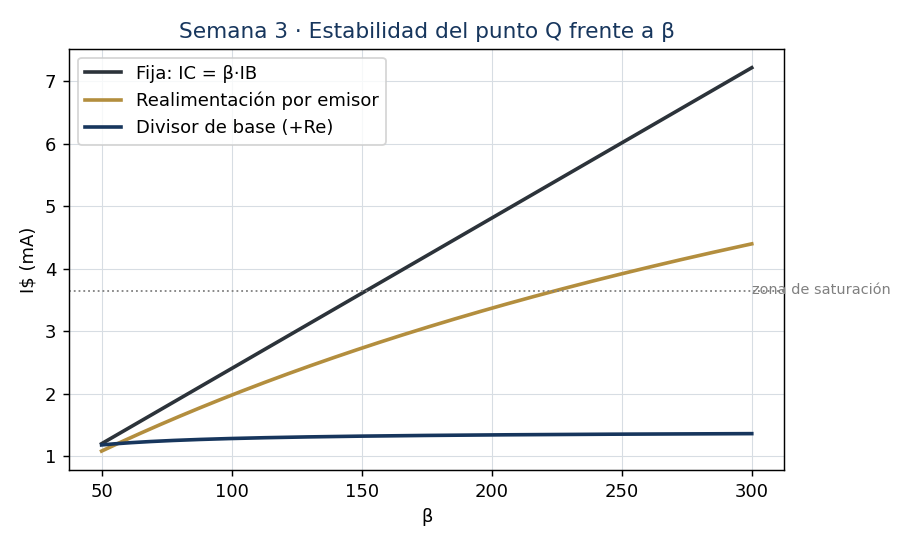
\includegraphics[width=0.72\textwidth]{figs/s3_estabilidad.png}
  \end{center}
  \begin{itemize}
    \item La \textbf{curva azul} (divisor de base) es casi \textbf{horizontal}:
      $I_C$ cambia muy poco al variar $\beta$. Es la topología \emph{más} estable.
    \item Por eso se usa para etapas que deben operar en un rango amplio de temperatura.
  \end{itemize}
\end{frame}

% ---------------------------------------------------------------------
\begin{frame}{Errores comunes}
  \begin{table}
    \small
    \begin{tabular}{p{0.34\textwidth}p{0.30\textwidth}p{0.30\textwidth}}
      \toprule
      Error & Consecuencia & Corrección \\
      \midrule
      Calcular $V_{th}$ con $R_1,R_2$ pero ignorar $R_{th}$ & Error de carga & $R_{th}$ entra en $I_E$ \\
      Asumir $V_{base} = V_{th}$ siempre & Ignorar caída en $R_{th}\cdot I_B$ & $I_E = (V_{th}-V_{BE})/(R_E+R_{th}/\beta)$ \\
      Olvidar $R_E$ en $V_{CE}$ & $V_{CE}$ erróneo & $V_{CE} = V_{CC}-I_C(R_C+R_E)$ \\
      Usar divisor "blando" ($R_{th}$ grande) & Inestabilidad & $R_{th}$ pequeño frente a $\beta R_E$ \\
      \bottomrule
    \end{tabular}
  \end{table}
\end{frame}

% ---------------------------------------------------------------------
\begin{frame}{Preguntas de verificación}
  \begin{enumerate}
    \item ¿Por qué el divisor de base es estable frente a $\beta$?
      \uncover<2->{\emph{($I_E \approx (V_{th}-V_{BE})/R_E$ no depende de $\beta$.)}}
    \item ¿Qué papel juega $R_{th}$ en el cálculo de $I_E$?
    \item Si $\beta$ cambia de 100 a 200, ¿cuánto cambia $I_C$ en esta topología?
      \uncover<3->{\emph{(Muy poco: $I_E$ casi constante.)}}
    \item ¿Qué ventaja tiene respecto de la polarización fija?
    \item ¿Cómo se relaciona $R_{th}$ del divisor con el equivalente de Thévenin de S2.4?
  \end{enumerate}
\end{frame}

\end{document}
